\section{Word Embeddings \label{ssec: word embeddings}}
    
    Word embeddings $\mathbf{w_i}$ are high-dimensional\footnote{word2vec by default uses 300 dimensional vectors.} vectors of real numbers aiming to represent the semantic meaning of a word $w_i$. Fig. \ref{fig: embeding graphic} gives a simple example of such embeddings. $\mathbf{w_i}$ are created by using large corpora of texts, (such as all Wikipedia articles, or a crawl through the entire internet) and using the context of words $w_i$ to learn their representation $\mathbf{w_i}$ in an unsupervised way. The basis for this is the assumption that similar words appear in similar contexts. Word embeddings are at the heart of many NLP applications and many pre-trained word embeddings are available. The most prominent are Google's, word2vec\cite{word2vec} and Stanford university's GloVe\cite{glove} embeddings, but the lesser known \textit{ConceptNet Numberbatch} embeddings\cite{conceptnet} build upon (and improve) both Glove and word2vec (see Sec. \ref{ssec: Numberbatch}).
    
    \subsection{GloVe \label{ssec: Glove}}
        GloVe\cite{glove} (short for Global Vectors) is a model 
        
        \[ \hat{f}(w_i) \rightarrow \mathbf{w_i}\] 
        
        for representing embeddings words as vectors. It is trained on very large corpora such as Wikipedia or a crawl of the entire internet. First, the co-occurence matrix $C_{ij}$ is created:
        
        \begin{equation}
        C_{ij} = \text{\# Co-occurences between words $i$ and $j$},
        \end{equation}
        
        where a co-occurence of two words means that they are featured within the same document, e.g. the same Wikipedia article or the same website. If there are $N_w$ words in the corpus, $C_{ij}$ is a $N_w \times N_w$ matrix, measuring the co-occurence between every word $w_i$ with every other word $w_j$. For GloVe, $N_w = \num{1.9e6}$ when trained on Wikipedia, $N_w = \num{2.2e6}$ when trained on a crawl of the entire internet. $C_{ij}$ is sparse, (meaning most entries are 0) as most words do not appear in the same context as most other words. By then performing dimensionality reduction (such as linear discriminant analysis) on $C_{ij}$, a dense representation of much lower dimensionality is obtained for every word. This representation is the word embedding. For GloVe, embeddings are by default 300-dimensional.\cite{glove}
        
        Word2vec is trained in a similar way, though what counts as a co-occurence and how the dimensionality is reduced is slightly different.
        
    \subsection{ConceptNet Numberbatch \label{ssec: Numberbatch}}
        
        ConceptNet is a open source semantic network that represents words (and short sequences of words commonly seen together) as nodes and the relationships between them as edges. An example is shown in Fig. \ref{fig: conceptnet}.
           \begin{figure}[h]
                \centering
                 \captionsetup{format=hang}
                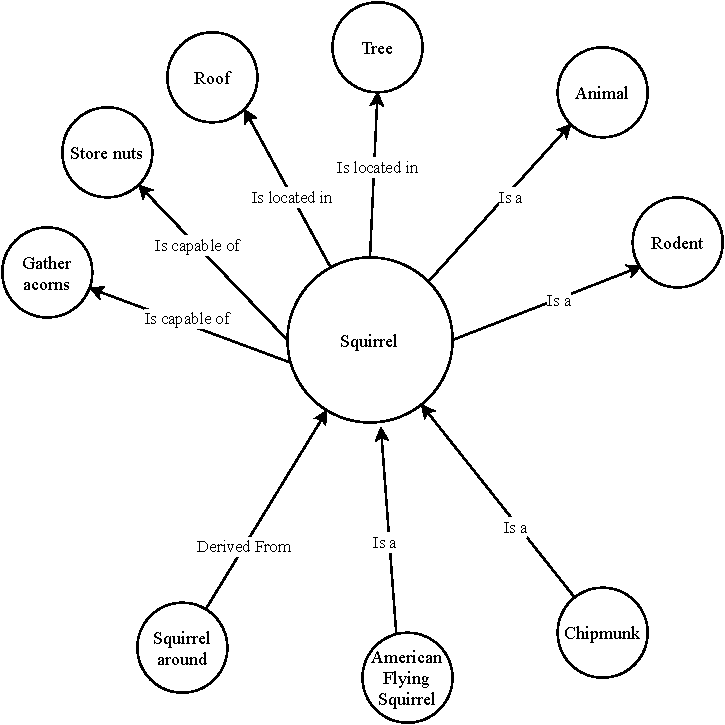
\includegraphics[width=0.7\textwidth]{conceptnet.pdf}
                \caption{Some of the connections of the word ``squirrel" in conceptNet. \label{fig: conceptnet}}
            \end{figure}
        
        By combining the ConceptNet network with other word embeddings such as word2vec and GloVe using a process called \textit{retrofitting}, a new, improved set of word embeddings, the \textit{Numberbatch}, is created.
        
        \subsubsection{Retrofitting}
            Retrofitting uses a set of embeddings $\mathbf{w_i}$, such as GloVe or word2vec (Sec. \ref{ssec: Glove}) to infer new embeddings $\Tilde{\mathbf{w_i}}$ that are both close to the original embeddings and also close to their neighbours in the ConceptNet graph, by minimising the objective function 
            \begin{equation}
                \Psi(W)=\sum_{i=1}^{N}\left[\alpha_{i}\left\|\mathbf{w}_{i}-\Tilde{\mathbf{w}}_{i}\right\|^{2}+\sum_{(i, j) \in E} \beta_{i j}\left\|\mathbf{w}_{i}-\mathbf{w}_{j}\right\|^{2}\right],
            \end{equation}
            
            where the sum is over all words included within the union of all words contained in ConceptNet with all words contained in the original embeddings, $W$ is the set of all word embeddings $\mathbf{w_i} \in W$, $E$ is the set of all edges within the ConceptNet graph, $\beta_{ij}$ is the weight of the edge between words $w_i$ and $w_j$ in the ConceptNet graph, and $\alpha_i$ are weights determining how important the previous embeddings are compared to the edges within ConceptNet. How exactly $\alpha_i$ is determined is not explained within the original paper, but when a word is found within ConceptNet, that was not found within the embeddings, $\alpha_i = 0$, allowing for a further expansion of the vocabulary.\cite{speer2017conceptnet}
        
        \subsubsection{Superior Performance}
            By combining word2vec, GloVe and ConceptNet, the ConceptNet Numberbatch achieves superior performance in many word embedding benchmarks. FIG ???.\cite{speer2017conceptnet, conceptnetPerformance}.
        
        \subsubsection{Mini Version}
            As a convenience, the Numberbatch embeddings are available as both more accurate 32-bit floating point numbers and as less accurate 8-bit integers. This allows for significantly smaller files (mini $\approx$ 50MB, full embeddings $\approx$ 5GB) and loading times. We use the mini versions due to limited resources.
        
    \subsection{Similarity \label{ssec: cosine similarity}} 
        The defining feature of word embeddings is that semantically similar words have similar vectors. We can thus quantify the similarity $\eta_{ij}$ between two words $w_i, w_j$ as the cosine similarity of their embeddings
        \begin{equation}
            \eta_{ij} = \frac{\mathbf{w_i} \cdot \mathbf{w_j}}{|\mathbf{w_i}| |\mathbf{w_j}|}.
            \label{eq: cosine similarity}
        \end{equation}
        We use this notion of similarity heavily in this work.
    
    \subsection{Sentence Embeddings \label{ssec: utterance embeddings}}
    
    In the same way that words can be embedded based on a pre-trained set of embeddings, sentences can be embedded also. Generating the embeddings doesn't work in the same way as for words (otherwise every sentence would have to be contained within the corpus for an embedding to exist), but the concept is the same. A sentence is represented as a vector in a high-dimensional vector space. This allows a similarity between sentences to be computed as the cosine similarity (see Sec. \ref{ssec: cosine similarity}, Eq. \ref{eq: cosine similarity}). Examples include Google's universal sentence encoder\cite{GoogleEncoder} and Facebook's InferSent\cite{infersent}.
     
    \subsection{Limitations}
        \begin{figure}[h]
            \centering
            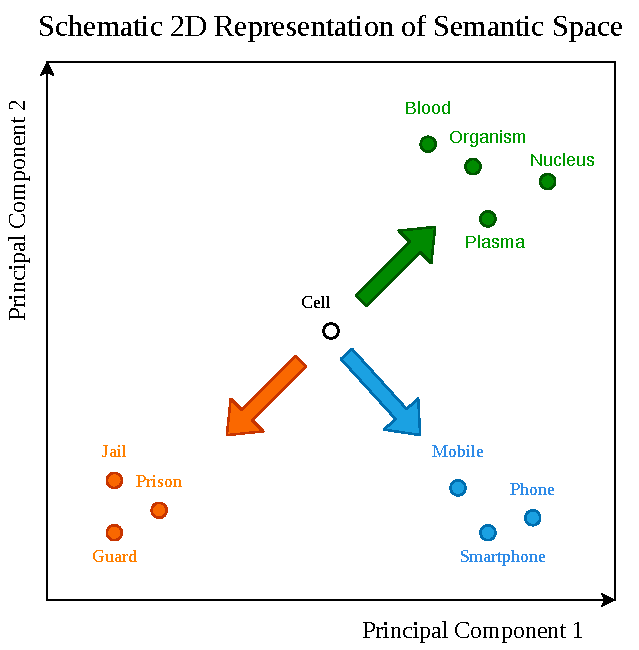
\includegraphics{ambiguous_embedding.pdf}
            \caption{Due to appearing frequently in contexts relating to biology, phones and prison, the word embedding for the ambiguous word ``cell" is attracted to all three contexts in semantic space. The final embedding lies somewhere in between the contexts and is a poor representation for all three meanings of ``cell".}
            \label{fig:ambiguous_embedding}
        \end{figure}
        
        Word embeddings suffer from some limitations, the most significant of which is the problem of word-sense disambiguation, which occurs because words may have multiple meanings but only one embedding. In the sentence
        \begin{align*}
            &\textit{``He went to the prison cell with his cell phone to extract blood cell samples}\\
            & \textit{from the inmates."}
        \end{align*}
        
        the word \textit{cell} appears 3 times and has a different meaning every time, but it has only one word embedding. Because the method of embedding is incapable of disambiguating the different meanings of the words, the word embedding is poor: In the semantic vector space of word embeddings, \textit{cell} will be attracted to words within its ``biology context", but also within its ``phone" context and within its ``prison" context, leading to a final embedding somewhere in the middle, making it ineffective within all three contexts. The newest types of word embeddings, such as BERT\cite{devlin2018bert} or ELMo\cite{peters2018elmo} address this problem by taking whole sentences as inputs and use the context of adjacent words to compute disambiguated word embeddings.